%%%%%%%%%%%%%%%%%%%%%%%%%%%%%%%%%%%%%%%%%%%%%%%%%%%%%%%%%%%%%%%%%%%%%%%%%%%%
% AGUtmpl.tex: this template file is for articles formatted with LaTeX2e,
% Modified December 2018
%
% This template includes commands and instructions
% given in the order necessary to produce a final output that will
% satisfy AGU requirements.
%
% FOR FIGURES, DO NOT USE \psfrag
%
%%%%%%%%%%%%%%%%%%%%%%%%%%%%%%%%%%%%%%%%%%%%%%%%%%%%%%%%%%%%%%%%%%%%%%%%%%%%
%
% IMPORTANT NOTE:
%
% SUPPORTING INFORMATION DOCUMENTATION IS NOT COPYEDITED BEFORE PUBLICATION.
%
%
%
%%%%%%%%%%%%%%%%%%%%%%%%%%%%%%%%%%%%%%%%%%%%%%%%%%%%%%%%%%%%%%%%%%%%%%%%%%%%
%
% Step 1: Set the \documentclass
%
%
% PLEASE USE THE DRAFT OPTION TO SUBMIT YOUR PAPERS.
% The draft option produces double spaced output.
%
% Choose the journal abbreviation for the journal you are
% submitting to:

% jgrga JOURNAL OF GEOPHYSICAL RESEARCH (use for all of them)
% gbc   GLOBAL BIOCHEMICAL CYCLES
% grl   GEOPHYSICAL RESEARCH LETTERS
% pal   PALEOCEANOGRAPHY
% ras   RADIO SCIENCE
% rog   REVIEWS OF GEOPHYSICS
% tec   TECTONICS
% wrr   WATER RESOURCES RESEARCH
% gc    GEOCHEMISTRY, GEOPHYSICS, GEOSYSTEMS
% sw    SPACE WEATHER
% ms    JAMES
% ef    EARTH'S FUTURE
%
%
%
% (If you are submitting to a journal other than jgrga,
% substitute the initials of the journal for "jgrga" below.)

\documentclass[draft,wrr]{../agutexSI2019}
\usepackage{amsmath}
% For using tabularx
\usepackage{tabularx}
\usepackage{booktabs}
%%%%%%%%%%%%%%%%%%%%%%%%%%%%%%%%%%%%%%%%%%%%%%%%%%%%%%%%%%%%%%%%%%%%%%%%%
%
%  SUPPORTING INFORMATION TEMPLATE
%
%% ------------------------------------------------------------------------ %%
%
%
%Please use this template when formatting and submitting your Supporting Information.

%This template serves as both a “table of contents” for the supporting information for your article and as a summary of files.
%
%
%OVERVIEW
%
%Please note that all supporting information will be peer reviewed with your manuscript. It will not be copyedited if the paper is accepted.
%In general, the purpose of the supporting information is to enable authors to provide and archive auxiliary information such as data tables, method information, figures, video, or computer software, in digital formats so that other scientists can use it.
%The key criteria are that the data:
% 1. supplement the main scientific conclusions of the paper but are not essential to the conclusions (with the exception of
%    including %data so the experiment can be reproducible);
% 2. are likely to be usable or used by other scientists working in the field;
% 3. are described with sufficient precision that other scientists can understand them, and
% 4. are not exe files.
%
%USING THIS TEMPLATE
%
%***All references should be included in the reference list of the main paper so that they can be indexed, linked, and counted as citations.  The reference section does not count toward length limits.
%
%All Supporting text and figures should be included in this document. Insert supporting information content into each appropriate section of the template. To add additional captions, simply copy and paste each sample as needed.

%Tables may be included, but can also be uploaded separately, especially if they are larger than 1 page, or if necessary for retaining table formatting. Data sets, large tables, movie files, and audio files should be uploaded separately. Include their captions in this document and list the file name with the caption. You will be prompted to upload these files on the Upload Files tab during the submission process, using file type “Supporting Information (SI)”

%IMPORTANT NOTE ON FIGURES AND TABLES
% Placeholders for figures and tables appear after the \end{article} command, after references.
% DO NOT USE \psfrag or \subfigure commands.
%
 \usepackage{graphicx}
%
%  Uncomment the following command to allow illustrations to print
%   when using Draft:
\setkeys{Gin}{draft=true}
%
% You may need to use one of these options for graphicx depending on the driver program you are using.
%
% [xdvi], [dvipdf], [dvipsone], [dviwindo], [emtex], [dviwin],
% [pctexps],  [pctexwin],  [pctexhp],  [pctex32], [truetex], [tcidvi],
% [oztex], [textures]
%
%
%% ------------------------------------------------------------------------ %%
%
%  ENTER PREAMBLE
%
%% ------------------------------------------------------------------------ %%

% Author names in capital letters:
%\authorrunninghead{BALES ET AL.}

% Shorter version of title entered in capital letters:
%\titlerunninghead{SHORT TITLE}

%Corresponding author mailing address and e-mail address:
%\authoraddr{Corresponding author: A. B. Smith,
%Department of Hydrology and Water Resources, University of
%Arizona, Harshbarger Building 11, Tucson, AZ 85721, USA.
%(a.b.smith@hwr.arizona.edu)}

\begin{document}
\noindent\textbf{\large{Supplementary Information for}}

%\includegraphics{agu_pubart-white_reduced.eps}

\graphicspath{{/Users/songshgeo/Documents/VSCode/WGRegimes_YRB_2020/figures}}
\title{Identifying regime transitions for water governance at the Yellow River Basin, China}
%
% e.g., \title{Supporting Information for "Terrestrial ring current:
% Origin, formation, and decay $\alpha\beta\Gamma\Delta$"}
%
%DOI: 10.1002/%insert paper number here%

%% ------------------------------------------------------------------------ %%
%
%  AUTHORS AND AFFILIATIONS
%
%% ------------------------------------------------------------------------ %%


% List authors by first name or initial followed by last name and
% separated by commas. Use \affil{} to number affiliations, and
% \thanks{} for author notes.
% Additional author notes should be indicated with \thanks{} (for
% example, for current addresses).

% Example: \authors{A. B. Author\affil{1}\thanks{Current address, Antartica}, B. C. Author\affil{2,3}, and D. E.
% Author\affil{3,4}\thanks{Also funded by Monsanto.}}

\authors{
      Shuang Song\affil{1},
      Shuai Wang\affil{1},
      Xutong Wu\affil{1},
      yongping Wei\affil{2},
      Graeme S. Cumming\affil{3},
      Yue Qin\affil{4},
      Xilin Wu\affil{5},
      Bojie Fu\affil{1,5}
}


\affiliation{1}{
      State Key Laboratory of Earth Surface Processes and Resource Ecology,
      Beijing Normal University,
      Beijing, 100875, Beijing, China.
}
\affiliation{2}{
      School of Earth and Environmental Sciences,
      The University of Queensland,
      Brisbane, 4067, QLD, Australia.
}
\affiliation{3}{
      ARC Centre of Excellence for Coral Reef Studies,
      James Cook University,
      Townsville, 4811, QLD, Australia.
}
\affiliation{4}{
      College of Environmental Sciences and Engineering,
      Peking University,
      Beijing, 100875, Beijing, China.
}
\affiliation{5}{
      State Key Laboratory of Urban and Regional Ecology,
      Research Center for Eco-Environmental Sciences,
      Chinese Academy of Sciences,
      Beijing, 100875, Beijing, China.
}

\begin{article}

\noindent\textbf{Contents of this file}
%%%Remove or add items as needed%%%
\begin{enumerate}
\item Text S1 to S4
\item Figures S1 to Figure~\ref{fig:recent}
%if Tables are larger than 1 page, upload as separate excel file
\end{enumerate}

\noindent\textbf{Introduction}
%Type or paste your text here. The introduction gives a brief overview of the supporting information. You should include information %about as many of the following as possible (when appropriate):
% 1. a general overview of the kind of data files;
% 2. information about when and how the data were collected or created;
% 3. a general description of processing steps used;
% 4. any known imperfections or anomalies in the data.
Section~\ref{secA1} provides a brief introduction to four regions (Source Region, Upper Region, Middle Region, and Lower Region -SR, UR, MR, and LR) of the YRB.\
Section~\ref{secA2} detailed explains the changing trend of three indicators.
Section~\ref{secA3} describes the correlations between the three indicators and
Section~\ref{secA4} provides some sensitivity analysis for testing robustness.

% Based on vary characteristics, we divide the YRB into four regions: source region (SR), upper region (UR), middle region (MR), and lower region (LR), according to characteristics and customary practices in the~\ref{secA1}.

\noindent\textbf{S1. YRB Regions}\label{secA1}
We divide the YRB into four regions to calculate the indicators considering both socio-economic and natural conditions. The division aligns with the customary schema from publications and the YRCC~\cite{yellowriverconservancycommission2013,wang2019c,wang2016e}, so four important hydrological stations can distinguish the regions (see Figure~\ref{fig:YRB}).

\begin{itemize}
    \item \textbf{Source Region (SR):} Over 50\% of natural runoff originates from this region. The most ecological function here is water yield, as sparsely populated and less economically developed.
    \item \textbf{Upper Region (UR):} With the highest per capita irrigated land area, there are numbers of large irrigation lands in this region. However, irrigation efficiency is relatively much lower than its lower reaches.
    \item \textbf{Middle Region (MR):} Crossing Loess Plateau, a famous rich-sand area, Yellow River loads most of its sediments here with the highest soil erosion risk. The ``grain for the green'' project changed the water utilization here strikingly to reverse this situation~\cite{wu2020a}.
    \item \textbf{Lower Region (LR):} With a dense population and the traditional agricultural trajectory, the lower region used to be the largest water use region. However, as the industrial transformation going, the proportion of agriculture keeps decreasing, but LR is still the largest water use region in each aspect.
\end{itemize}

% 补充图片1:研究区示意图
\begin{figure*}[hbtp!]
    \centering
    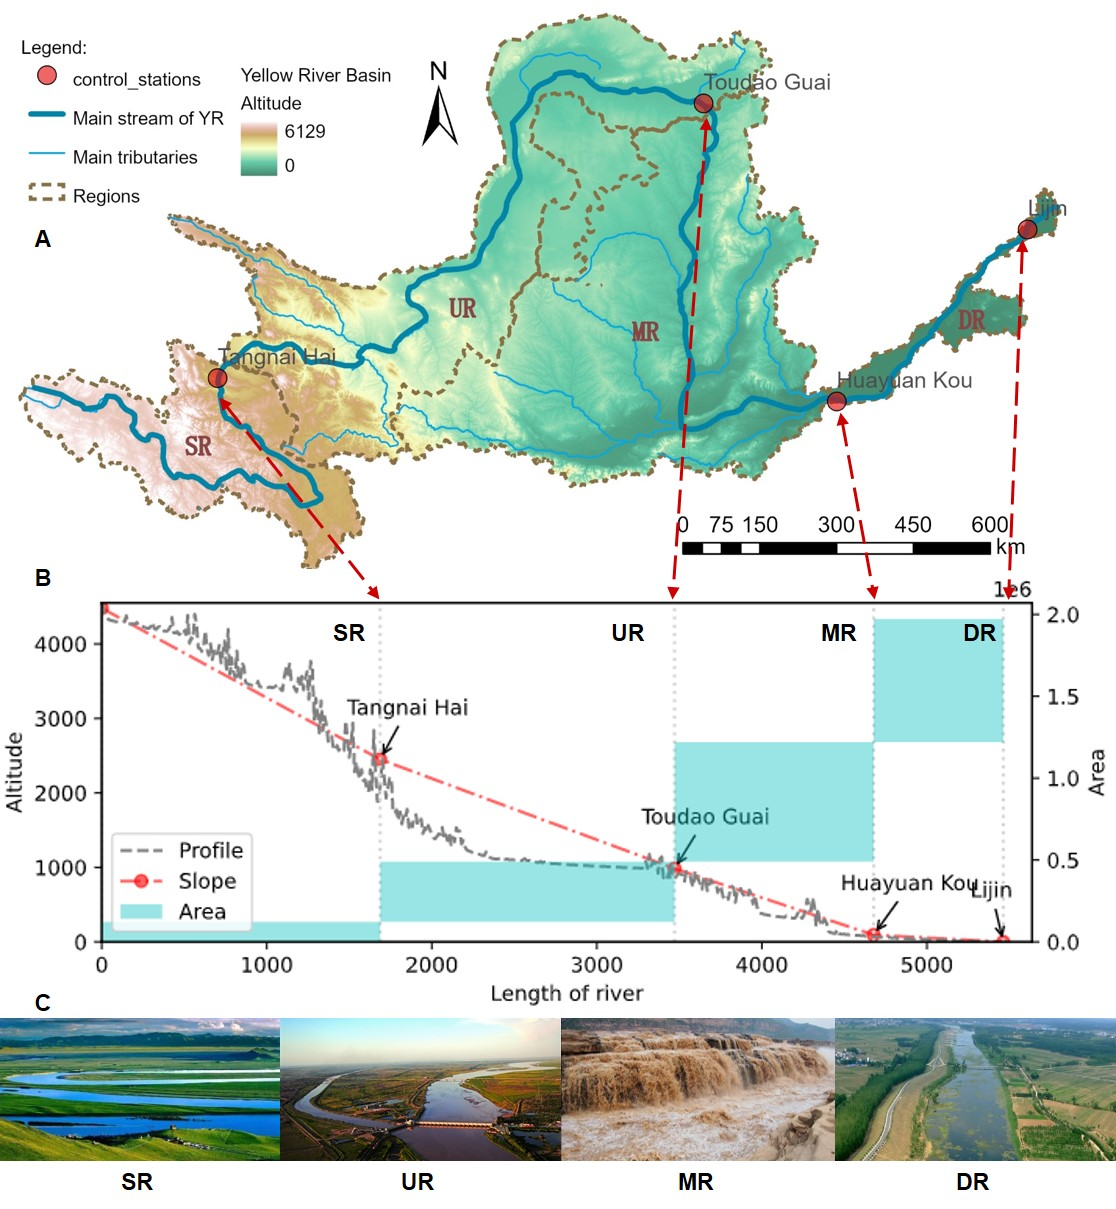
\includegraphics[width=0.6\textwidth]{sup/s1_study_area.jpg}
    \caption{
        The study area.
        \textbf{A.} Diagram of the YRB and the subdivision of the basin (SR: Source Region, UR: Upper Region, MR: Middle Region, DR: Downstream region).
        \textbf{B.} Profile of the main channel of the Yellow River. The hydrological stations control the SR, UR, MR and DR.
        \textbf{C.} Typical landscapes in different regions in the YRB.
    }\label{fig:YRB}
\end{figure*}

% % 补充图片4:天然水资源量
% \begin{figure*}[tb]
%     \centering
%     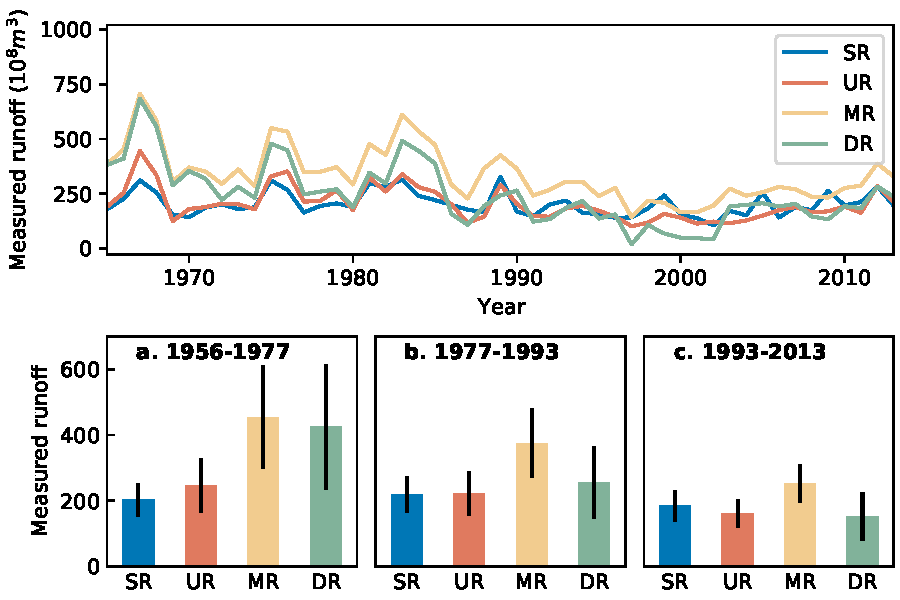
\includegraphics[width=0.8\textwidth]{sup/sf_measured_runoff.pdf}
%     \caption{Water resources in different regions.
%         \textbf{A,} changing trend of measured runoff,
%         \textbf{B, C and D} average measured runoff within different periods.
%         \textbf{E, F and G} average total water consumptions within different periods.
%     }
%     \label{fig:water resources}
% \end{figure*}


\noindent\textbf{S2. Trend of Indicators}\label{secA2}
By taking water flexibility and variability into account, the scarcity-flexibility-variability (SFV) index focus more on dynamic responses to water resources in a developing perspective, which is a valid metric of temporal changes in water stresses \cite{qin2019}. To apply this method, we need to combine three metrics following:

First, for scarcity, $A_{i, j}$ is the total water consumption as a proportion of regional multi-year average runoff volume in year $j$ and region $i$ (in this study, four regions in the YRB, \\textit{Supporting Information}~\ref{secA1}):
\begin{equation}
    A_{i, j} = \frac{WU_{i,j}}{R_{i, avg}}
\end{equation}

Second, for flexibility, $B_{i, j}$ is the inflexible water use $WU_{inflexible}$ (i.e. for thermal power plants or humans and livestock) as a proportion of average multi-year runoff, in year $i$ and region $j$:
\begin{equation}
    B_{i, j} = \frac{WU_{i, j, inflexible}}{R_{i, avg}}
\end{equation}

Finally for variability, the capacity of the reservoir and the positive effects of storage on natural runoff fluctuations are also considered.
\begin{gather}
C_i = C1_i * (1 - C2_i) \\
C1_{i, j} = \frac{R_{i, std}}{R_{i, avg}} \\
C2_{i} = \frac{RC_{i}}{R_{i, avg}}, \ if RC < R_{i, avg} \\
C2_{i} = 1, \ if RC >= R_{i, avg}
\end{gather}

In all the equations above, $R_{i, avg}$ is the average runoff in region $i$, $RC_i$ is the total storage capacities of reservoirs in the region $i$, $R_{i, std}$ is the standard deviation of runoff in the region $i$.

Finally, assuming three metrics (scarcity, flexibility and variability) have the same weights, we can calculate the $SFV$ index after normalizing them:
\begin{gather}
    V = \frac{A_{normalize} + B_{normalize} + C_{normalize}}{3}\\
    a = \frac{1}{V_{max} - V_{min}};\\
    b = \frac{1}{V_{min} - V_{max}} * V_{min}\\
    SFV = a * V + b
\end{gather}


\noindent\textbf{S3. Correlation of Indicators}\label{secA3}
% chktex-file 46

By analyzing the correlation of the integrated management index (IWGI) and its three sub-indexes: stress (IS), purpose (IP) and allocation (IA) in three different periods, namely, the massive supply regime (P1: $1965 \sim 1978$), governance transforming regime (P2: $1979 \sim 2001$) and adaptation oriented regime (P3: $2002 \sim 2013$), the following results are obtained.

When we focus on the correlation from P1 to P3, the results show significant negative correlation between IS and IP (correlation coefficient is $r = -0.75$, $p < 0.01$), indicating that there is a strong negative relationship between IS and IP.\
On the other hand, there is a significant positive correlation between IA and IWGI (correlation coefficients are $r = 0.75$, $p < 0.01$), indicating a positive relationship between IA and IWGI.\ However, the correlations of other combinations are not statistically significant overall.

The correlations between time periods are very different with the overall trend above.
There is no significant correlation between any indicator combinations in the massive supply regime (P1).
In the governance transforming regime (P2), there is a significant negative correlation between IS and IP (correlation coefficient $r = -0.90$, $p < 0.01$), a significant negative correlation between IS and IA (correlation coefficient $r = -0.87$, $p < 0.01$), and a significant positive correlation between IP and IA (correlation coefficient $r = 0.77$, $p < 0.01$).
The correlations between IS and IP, IS and IA, and IS and IWGI were not statistically significant in the adaptation oriented regime (P3). However, there is a significant negative correlation between IP and IA (correlation coefficients are $r = -0.86$, $p < 0.01$).

% Table generated by Excel2LaTeX from sheet '相关性情况'
\begin{table}[htbp]
    \centering
    \caption{The correlation of the Integrated Governance Index (IWGI) and its three sub-indicators (IS, IP, IA)}
      \begin{tabularx}{\textwidth}{XXXXXXX}
      \toprule
      Period & \multicolumn{1}{l}{IS vs IP} & \multicolumn{1}{l}{IS vs IA} & IP vs IA & \multicolumn{1}{l}{IP vs IWGI} & \multicolumn{1}{l}{IA vs IWGI} & \multicolumn{1}{l}{IS vs IWGI} \\
      \midrule
      P1 to P3 & \multicolumn{1}{l}{-0.75 *} & -0.29 & 0.36 & 0.37  & \multicolumn{1}{l}{0.75 *} & 0.14 \\
      P1    & -0.08 & -0.31 & 0.06 & 0.14  & 0.51  & 0.65 \\
      P2    & \multicolumn{1}{l}{-0.90 *} & \multicolumn{1}{l}{-0.87 *} & 0.77 * & -0.18 & -0.13 & 0.5 \\
      P3    & 0     & -0.38 & -0.86 * & -0.33 & 0.61  & 0 \\
      \bottomrule
      \end{tabularx}%
    \label{tab:corr}%
\end{table}%



\noindent\textbf{S4. Robustness}\label{secA4}
% 为了增强本研究的鲁棒性,我们在不同的显著性水平下检验了突变点的识别结果,发现在0.0005到0.05的置信度水平下,都只能识别出本研究发现的两个突变点(1978与2001)。
In order to enhance the robustness of this study, we tested the identification results of mutation points at different significance levels.
Our results that only two mutation points (1978 and 2001) could be identified at the confidence level of $0.0005$ to $0.05$ (Figure~\ref{fig:sensitivity}).
% 此外,我们讨论了在指标中没有体现的水库流量变化,在所有水库(图 x)中,我们分析了10个先后建成的枢纽水库,发现水库在 governance transforming regime 之后开始增强其调度的水平
In addition, we analyzed the changes of reservoir flow that are not reflected in the IWGI.\ Among all the reservoirs (Figure~\ref{fig:reservoirs}), we focused on $9$ major reservoirs built successively and find that the reservoirs began to enhance their variability after the governance transforming regime, suggesting a higher level of regulating (Figure~\ref{fig:conveyance}).

Last, we tried our best to strengthen the period of this study despite the limitations of time span of the multiple-source dataset. We calculated the IWGI from 2003 to 2017 by using data from Yellow River Water Resources Bulletin to extend the study period. Since our results suggest no significant regime change (Figure~\ref{fig:recent}), we think it is robust that the YRB experienced two significant water governance regime changes in 1978 and 2001, without further changing since 21th century.

\begin{figure}[tb]
    \centering
    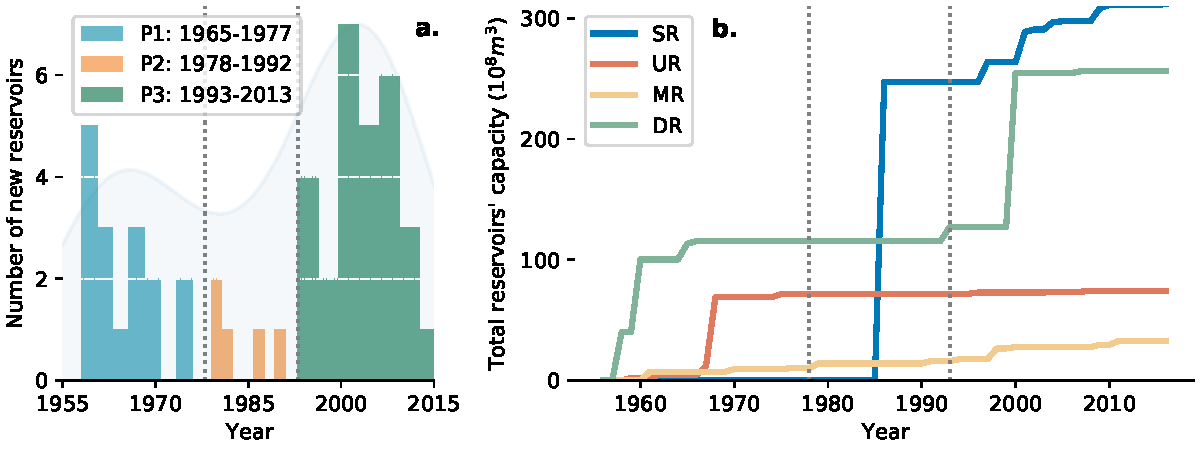
\includegraphics[width=0.6\linewidth]{sup/reservoirs.pdf}
    \caption{
          Numbers of new reservoirs in each year.
    }\label{fig:reservoirs}
\end{figure}

\begin{figure}
    \centering
    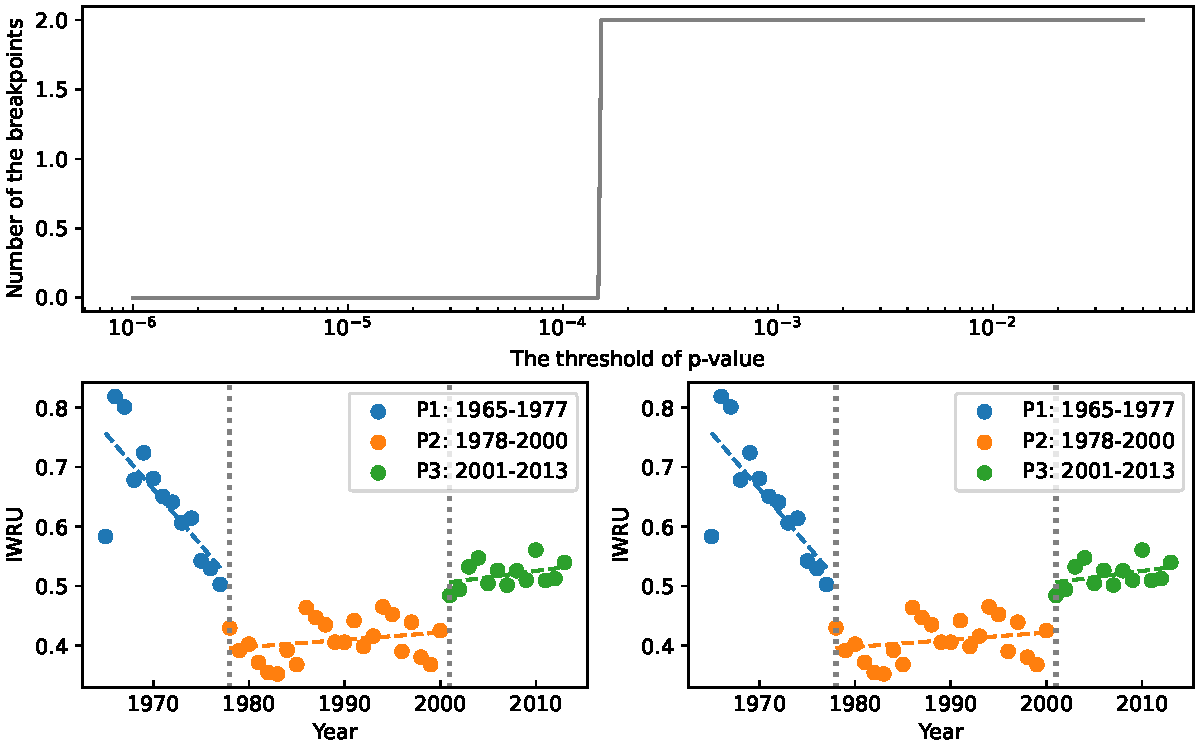
\includegraphics[width=\linewidth]{sup/sensitivity.pdf}
    \caption{
          Sensitivity analysis of the threshold of p-values.
          \textbf{A.} number of breakpoints in different p-values, the scheme with two-breakpoints are the dominant situation.
          \textbf{B.} Threshold of p-values \(\alpha=0.0005\).
          \textbf{C.} Threshold of p-values \(\alpha=0.05\).
    }\label{fig:sensitivity}
\end{figure}


\begin{figure}[htb]
    \centering
    \includegraphics[width=0.8\textwidth]{sup/conveyance.png}
    \caption{Monthly conveyance flow differences of the reservoirs mainly for managing and regulating the whole basin and their variability}\label{fig:conveyance}
\end{figure}


\begin{figure}[!htb]
	\centering
	\includegraphics[width=0.8\textwidth]{sup/robustness.png}
	\caption{Recent years' IWGI changes calculated by data from Yellow River Water Resources Bulletin. No significant changing point exists}\label{fig:recent}
\end{figure}



% \noindent\textbf{Datasets}\label{secA3}
% \subsection*{Descriptions}
This study used multiple types of data (see Table~\ref{tab:datasets}): statistical datasets, hydrological datasets, and political datasets.

\subsubsection*{Statistical datasets}
% We used GDP data; water resources uses data extracted from the 2nd National Water Resources Assessment Program \cite{zhou2020} and statistical yearbooks \url{http://www.yrcc.gov.cn/other/hhgb/}.
The water resources use dataset was published by Zhou et al. \cite{zhou2020}, which records water utilization in different sectors along with social-economic situations at the Prefectures level. 2nd National Water Resources Assessment Program mainly extracted this dataset launched in 2002, led by the National Development and Reform Commission and the Ministry of Water Resources (see ref (1) and \url{http://www.mwr.gov.cn/english/publs/} for more details). Since then, the statistics from the survey using the same criteria have been supplemented and harmonized with the 2013 administrative divisions.

The data covers a total of subcategories of water use under four broad categories: agriculture (IRR), industry (IND), urban (URB) and rural (RUR) water use (see Zhou et al., for details \cite{zhou2020}).
% There is uncertainty at the county scale for each disaggregated water use sector, but because the corrected data has been for statistical information using the water balance method, the data are adequate for the regional scale used in this study.

\subsubsection*{Hydrological datasets}
The reservoir dataset was collected by Wang et al. \cite{wang2019c}, which introduced includes the significant new reservoirs built in the YRB since 1949 (Figure~\ref{fig:reservoirs}). YRCC labelled the regulation-oriented reservoirs among them, see \url{http://www.yrcc.gov.cn/hhyl/sngc/}). In addition, annual runoff data derived from hydrological station measurements are the same as the datasets used in \cite{wang2019c} and \cite{wang2016e}.

\subsubsection*{Political datasets}
The policy dataset collects laws and policies listed in the book \cite{yellowriverconservancycommission2013}, which are related to the Yellow River basin promulgated and implemented by departments at (such as YRCC) and above (such as national institutions) at the Basin's level (Table~\ref{tab:policies}).
In addition, some are difficult to categorize; not a landmark, but numerous water governance practices in the YRB had been recorded in ``Yellow River Events'' by the YRCC; we collected them from \url{http://www.yrcc.gov.cn/hhyl/hhjs/}.

\subsection*{Methods S3. Harmonization}
Due to the wide sources of our data set and the different spatial scales, we need to harmonize them into a practical scale.
\begin{itemize}
    \item 1. Datasets at watersheds scales:
        We directly divided the annual hydrological data and measured runoff data according to their watersheds' corresponding hydrological stations (see Figure~\ref{fig:YRB} A and B).
    \item 2. Prefecture:
        We calculate the area of each prefecture to determine whether they belong to a region, with the threshold of $95\%$:

        \begin{equation}
            S_{ij} = MAX(S_ij / S_i)
        \end{equation}

        Where $i$ refers to a specific prefecture and $j$ refers to a region within YRB, i.e. SR, UR, MR, or DR. $S_i$ refers to the area of perfect $i$, and $S_{ij}$ refers intersecting area between perfect $i$ and region $j$.
        We define perfecture $i$ belongs to region $j$ if their intersecting area $S_{ij}$ over 95\% of $S_i$, i.e.:

        \begin{equation}
            MAX(S_{ij}) > 0.95 * S_i
        \end{equation}
    \item 3. Province:
        According to the major provinces contained in different regions, we determine which region the data of that province is merged into by referring to the traditional division practice:
    \begin{itemize}
        \item SR: Qinghai Gansu and Sichuan,
        \item UR: Ningxia and Inner Mongolia,
        \item MR: Shanxi and Shaanxi,
        \item DR: Shandong, Hebei and Henan.
    \end{itemize}
\end{itemize}

Finally, when we process the location data (i.e., the location data of the reservoirs), we judge the province it belongs to according to its location and then fit it to the regional scale.

\begin{table*}[!htbp]
    \begin{center}
    \small
    \begin{minipage}{\linewidth}
    \caption{Used datasets and their sources.}\label{tab:datasets}%
    \resizebox{\linewidth}{!}{
    \begin{tabular}{lrrrp{0.4\linewidth}}
    \toprule
    Dataset & Type & Spatial scale & Time scale & Source \\
    \midrule
    1. Administrative water use & Statistical & Prefectures & 1965-2013 & 2nd National Water Resources Assessment Program \cite{zhou2020}\\
    2. GDP & Statistical & Province & 1949-2019 & Wind database \\
    3. Streamflow withdrawals & Statistical & Watershed & 2003-2019 & Yearbooks \url{http://www.yrcc.gov.cn/other/hhgb/} \\
    4. Reservoirs & Hydrological & Location & 1949-2015 & Publication \cite{wang2019c} \\
    5. Measured runoff & Hydrological & Location & 1949-2019 & Measured data \cite{wang2019c,wang2016e} \\
    6. Laws & Political & Documents & 1949-2013 & YRCC \cite{yellowriverconservancycommission2013} \\
    7. History of YRCC & Political & Documents & 1949-2002 & YRCC \cite{yellowriverarchives2004} \\
    8. YRB Events & Political & Documents & 1949-2015 & YRCC: \url{http://www.yrcc.gov.cn/hhyl/hhjs/} \\
    \botrule
    \end{tabular}}
    \end{minipage}
    \end{center}
    \end{table*}

    %% 表格
\begin{table*}
    \centering
    \small
    \caption{Policies and regulations above YRB level which affected the whole basin in water utilization}\label{tab:policies}
    \begin{minipage}{\linewidth}
    \resizebox{\linewidth}{!}{
    \begin{tabular}{p{0.6\linewidth}rp{0.35\linewidth}}
        Name & Year & Agency \\
        \midrule
        1. Water Law of PRC & 1988 & National People's Congress of the PRC \\
        2. Water Law of PRC -revised 1 & 2009 & National People's Congress of the PRC \\
        3. Water Law of PRC -revised 2 & 2016 & National People's Congress of the PRC \\
        4. Regulations on the Administration of Water Drawing Licences and The Collection of water resource fees & 2006 & State Council of the PRC \\
        5. Regulations on the Administration of Water Drawing Licences and The Collection of water resource fees -revised 1 & 2017 & State Council of the PRC \\
        6. Regulations on the Allocation of Water in the Yellow River & 2006 & State Council of the PRC \\
        7. Yellow River water supply distribution scheme & 1987 & State Council of the PRC \\
        8. Measures for the Administration of Water Drawing Permits & 2008 & Ministry of Water Resources of the PRC \\
        9. Measures for the Administration of Water Drawing Permits -revised 1 & 2015 & Ministry of Water Resources of the PRC \\
        10. Measures for the Administration of Water Drawing Permits -revised 2 & 2017 & Ministry of Water Resources of the PRC \\
        11. Regulations on the Allocation of Water in the Yellow River & 2006 & State Council of the PRC \\
        12. Annual distribution of available water supply of the Yellow River and mainstream water dispatching scheme & 1998 & Ministry of Water Resources of the PRC \\
        13. The Yellow River water dispatching management measures & 1998 & Ministry of Water Resources \\
        14. Measures for the Implementation of the Yellow River Water Rights Conversion Management & 2004 & Ministry of Water Resources \\
        15. Regulations on the Administration of Water Drawing Licences and The Collection of water resource fees & 2006 & State Council of the PRC \\
        16. Measures for the implementation of the water drawing Permit system & 1993 \\ State Council of the PRC \\
        17. Measures for the demonstration and management of water resources in construction projects & 2002 & Ministry of Water Resources of the PRC \\
        18. Implementation Opinions on the Reform of Water Conservancy Project Management System & 2006 & State Council of the PRC \\
        \bottomrule
    \end{tabular}}

    \footnotesize[1]{If a policy was proposed by multiple legacies, we only show the highest one.}
    \end{minipage}
\end{table*}


%%Enter Data Set, Movie, and Audio captions here
%%EXAMPLE CAPTIONS

% \noindent\textbf{Data Set S1.} %Type or paste caption here.
%upload your dataset(s) to AGU's journal submission site and select "Supporting Information (SI)" as the file type. Following naming %convention: ds01.

%Repeat for any additional Supporting data sets

% \noindent\textbf{Movie S1.} %Type or paste caption here.
%upload your movie(s) to AGU's journal submission site and select, "Supporting Information %(SI)" as the file type. Following naming convention: ms01.

%Repeat any additional Supporting movies

% \noindent\textbf{Audio S1.} %Type or paste caption here.
%upload your audio file(s) to AGU's journal submission site and select "Supporting Information %(SI)" as the file type. Following naming convention: auds01.


%Repeat for any additional Supporting audio files

%%% End of body of article:
%%%%%%%%%%%%%%%%%%%%%%%%%%%%%%%%%%%%%%%%%%%%%%%%%%%%%%%%%%%%%%%%
%
% Optional Notation section goes here
%
% Notation -- End each entry with a period.
% \begin{notation}
% Term & definition.\\
% Second term & second definition.\\
% \end{notation}
%%%%%%%%%%%%%%%%%%%%%%%%%%%%%%%%%%%%%%%%%%%%%%%%%%%%%%%%%%%%%%%%


%% ------------------------------------------------------------------------ %%
%%  REFERENCE LIST AND TEXT CITATIONS

%%%%%%%%%%%%%%%%%%%%%%%%%%%%%%%%%%%%%%%%%%%%%%%
%
%
\bibliography{../mybibtex.bib}
\end{article}
\clearpage
\end{document}
